\section{Tape-Out}
\label{sec:tapout}

We intended to finish the chip design portion of this project in the previous thesis, however slip in the timeline caused us to miss the first tape-out deadline and submission date for that thesis. A large part of the slippage was caused by having to redesign the buck-boost converter regulator loop to implement peak current-mode control due to issues with the previously implemented average current-mode control. Even with the extended timeline it was difficult to complete the design before the deadline leading us rush some aspects of the design and remove nonessential features like the over-temperature protection circuit we designed.

\subsection{Buck-Boost Converter}
The layout of the buck-boost converter can be seen in  \autoref{fig:BBlayout} with annotations showing the rough floorplan the block. Surrounding the converter are the four large transistors.


\begin{figure}[h]
    \centering
    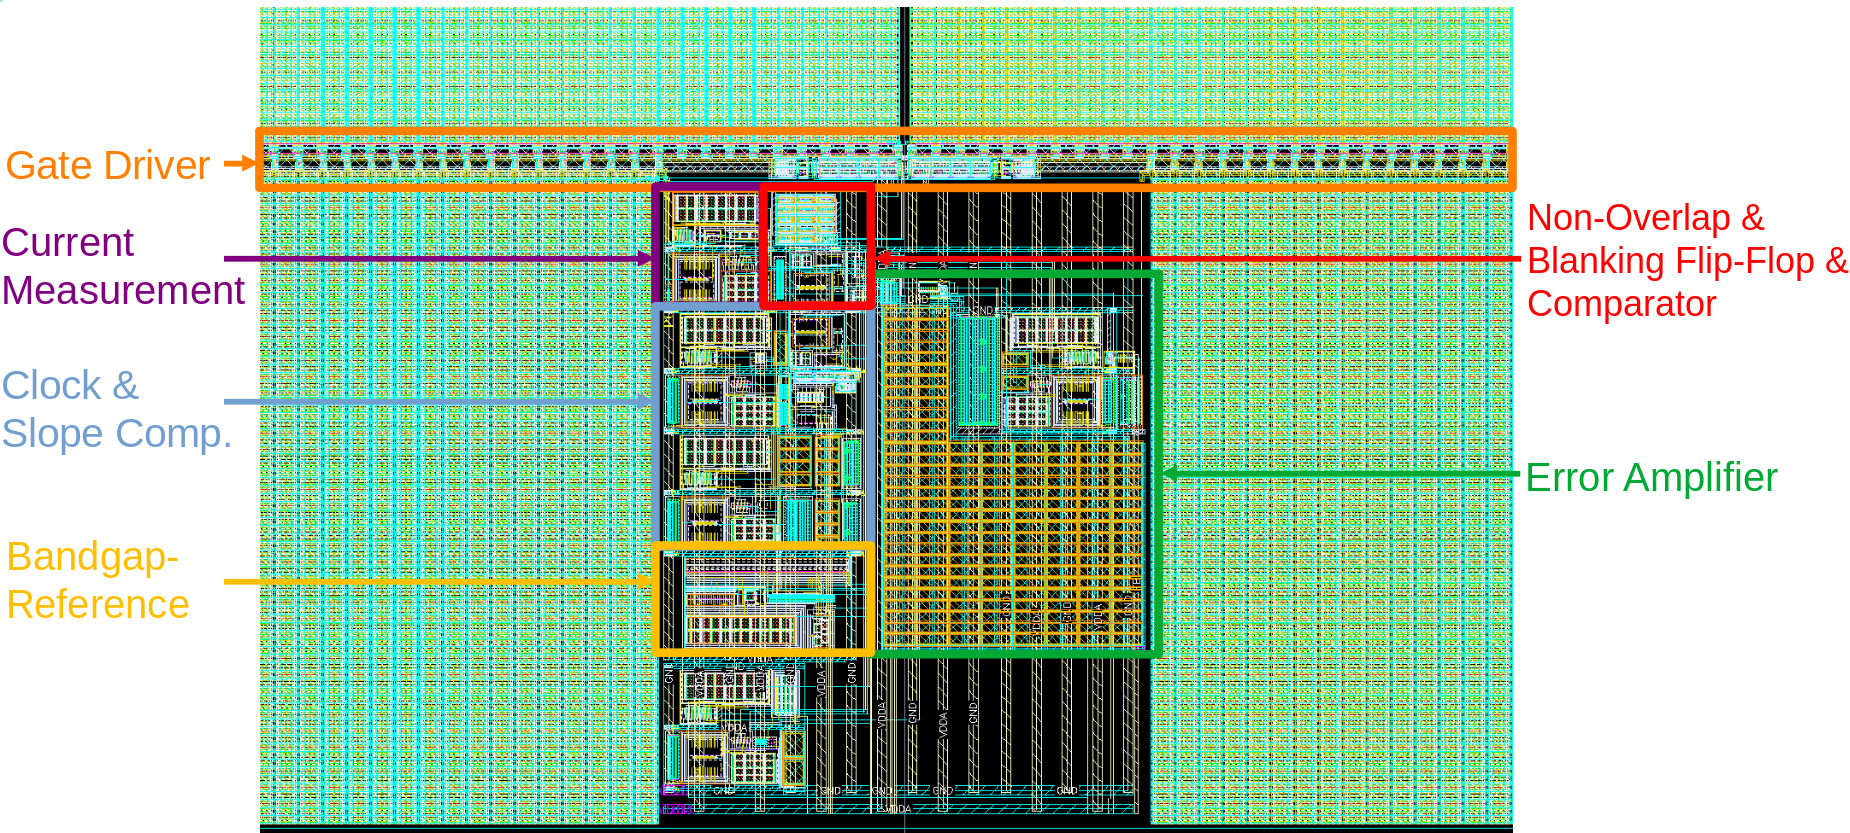
\includegraphics[width=1\textwidth]{../ASIC-DESIGN-2/images/07_DCDC/BuckBoostLayout.png}
    \caption{Layout of the buck-boost converter regulator surrounded by the large power stage transistors}
    \label{fig:BBlayout}
\end{figure}

\subsection{Overall Chip Floorplan}
\begin{figure}[h]
    \centering
    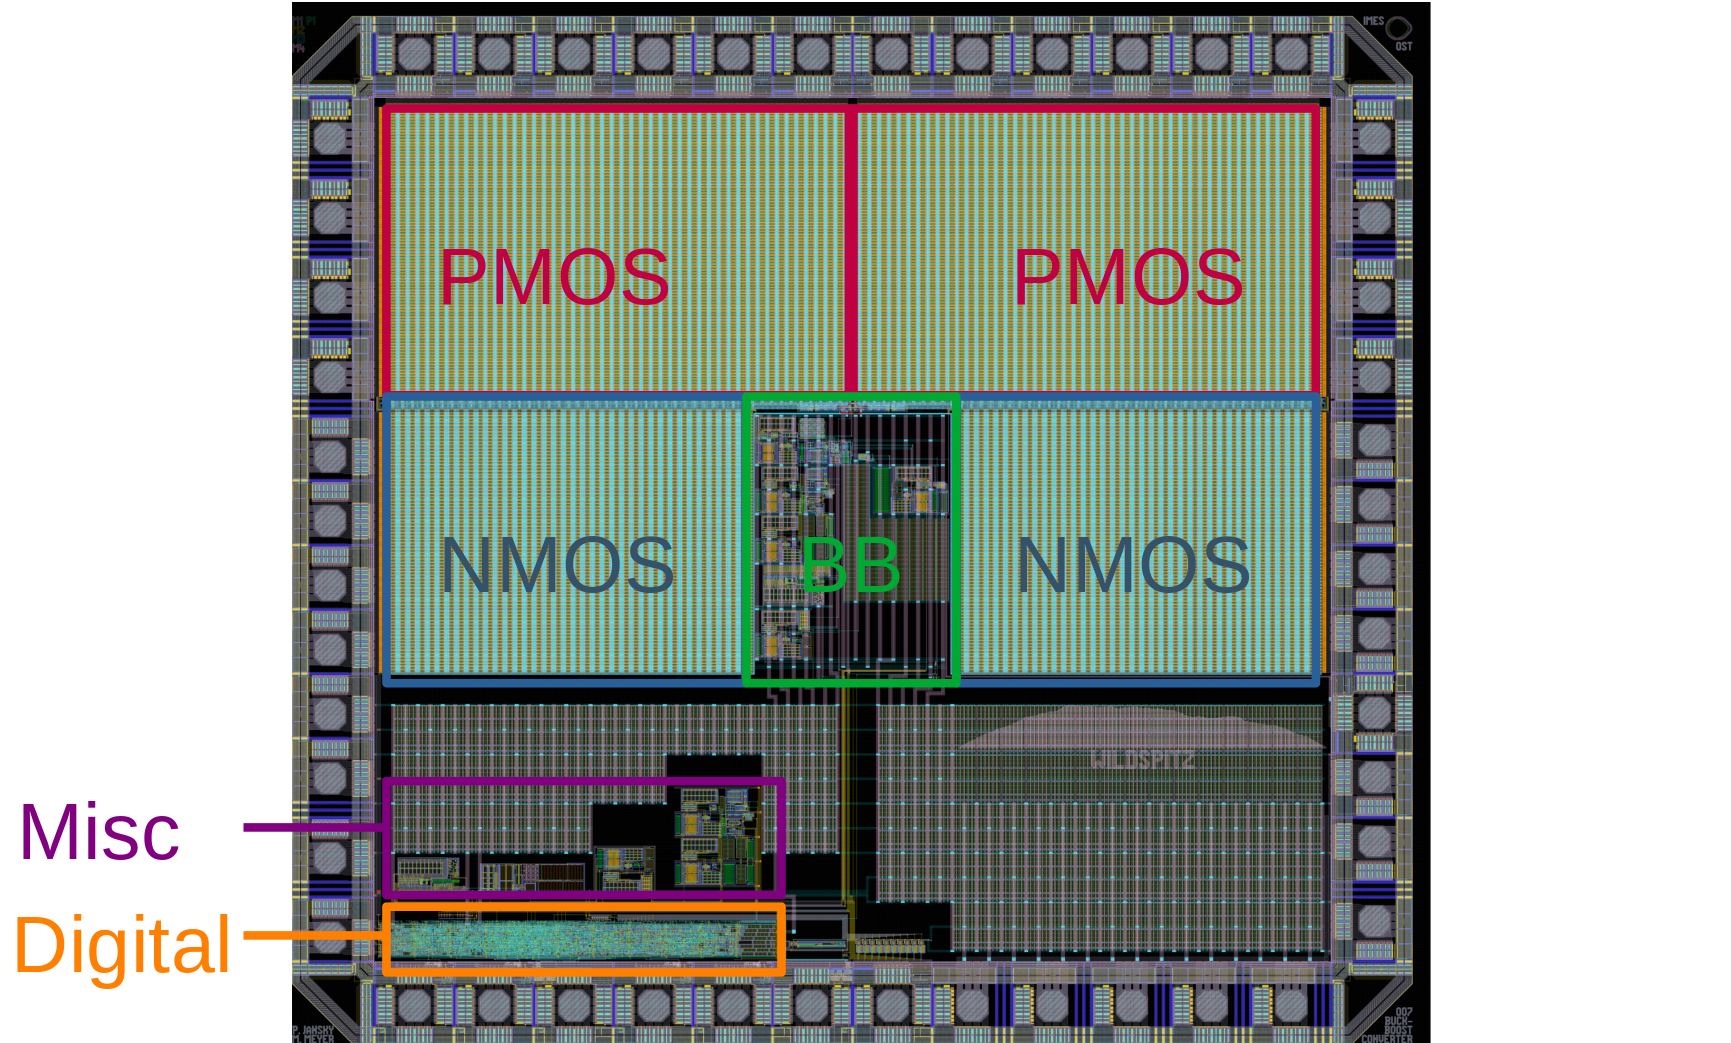
\includegraphics[width=1\textwidth]{../ASIC-DESIGN-2/images/07_DCDC/ChipLayout.png}
    \caption{Layout of the buck-boost converter regulator surrounded by the large power stage transistors}
    \label{fig:chiplayout}
\end{figure}

